% KYBELE: the expertise sits in the orchestrator, not in the model.
% ---------------------------------------------------------------------------
% style.tex --- shared preamble for every figure in book/figures/tikz/
%
% One style for all figures: Latin Modern, thin black lines, a light grey
% fill, and one accent colour used only to mark what is untrusted or wrong.
% Build with scripts/build_figures.sh; see book/figures/README.md.
% ---------------------------------------------------------------------------
\documentclass[tikz,border=6pt]{standalone}
\usepackage[T1]{fontenc}
\usepackage{lmodern}
\usetikzlibrary{arrows.meta,positioning,shapes.geometric,calc,fit,backgrounds}

\hyphenpenalty=10000   % short lines in boxes: ragged, never hyphenated

\definecolor{lightgrey}{gray}{0.92}
\definecolor{accent}{HTML}{9B2D20}

\tikzset{
  every picture/.style={
    line width=0.6pt,
    font=\small,
    >={Stealth[length=5pt,width=4pt]},
    node distance=14pt and 24pt,
  },
  % shapes
  box/.style={draw, rectangle, inner xsep=8pt, inner ysep=5pt,
              minimum height=22pt, align=center},
  grey/.style={box, fill=lightgrey},
  rounded/.style={box, rounded corners=9pt},
  decision/.style={draw, diamond, aspect=2.4, inner sep=1.5pt, align=center},
  group/.style={draw, dashed, rounded corners=5pt, inner sep=7pt},
  % text
  tag/.style={font=\footnotesize, align=center, inner sep=2pt},
  note/.style={font=\footnotesize\itshape, align=center, inner sep=2pt},
  code/.style={font=\small\ttfamily},
  codetag/.style={font=\footnotesize\ttfamily, align=center, inner sep=2pt},
  title/.style={font=\small\scshape, align=center, inner sep=2pt},
  % lines
  arrow/.style={->},
  back/.style={->, dashed},
  thin/.style={line width=0.4pt, gray},
  % the one accent, for what is untrusted, wrong or missing
  bad/.style={accent},
  badbox/.style={box, draw=accent, text=accent},
}

\begin{document}
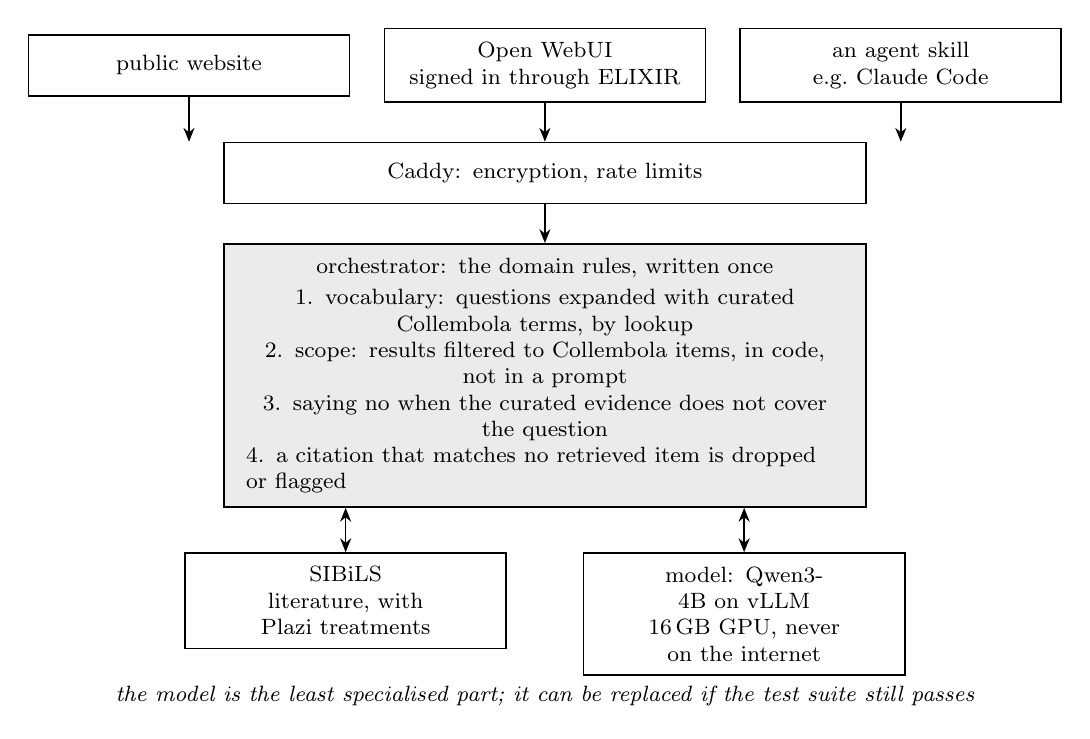
\begin{tikzpicture}[node distance=14pt and 12pt, part/.style={box, text width=100pt, align=center, font=\footnotesize}]
  \node[part] (web) {public website};
  \node[part, right=of web] (ui) {Open WebUI\\signed in through ELIXIR};
  \node[part, right=of ui] (skill) {an agent skill\\e.g.\ Claude Code};
  \node[box, below=of ui, text width=216pt, align=center, font=\footnotesize] (caddy) {Caddy: encryption, rate limits};
  \node[grey, below=of caddy, text width=216pt, align=left, font=\footnotesize] (orch)
    {\centering orchestrator: the domain rules, written once\\[2pt]
     1. vocabulary: questions expanded with curated Collembola terms, by lookup\\
     2. scope: results filtered to Collembola items, in code, not in a prompt\\
     3. saying no when the curated evidence does not cover the question\\
     4. a citation that matches no retrieved item is dropped or flagged};
  \node[part, below=16pt of orch.south, anchor=north, xshift=-72pt] (sibils) {SIBiLS\\literature, with Plazi treatments};
  \node[part, below=16pt of orch.south, anchor=north, xshift=72pt] (model) {model: Qwen3-4B on vLLM\\16\,GB GPU, never on the internet};
  \foreach \c in {web,ui,skill} \draw[->] (\c) -- (\c |- caddy.north);
  \draw[->] (caddy) -- (orch);
  \draw[<->] (orch.south -| sibils.north) -- (sibils.north);
  \draw[<->] (orch.south -| model.north) -- (model.north);
  \node[note] at ($(sibils.south)!0.5!(model.south)+(0,-12pt)$) {the model is the least specialised part; it can be replaced if the test suite still passes};
\end{tikzpicture}
\end{document}
